\chapter{Stochastic Differential Equations}
\label{ch-stochastic-diff-eqns}

This chapter is based mostly on Ref.\cite{sar-sol}.

{\bf Stochastic Differential Equations (SDE)}
are deterministic first order differential equations with additive external white noise. When discretized, they 
can be modelled as dynamic bnets of type
DEN (Deterministic bnet with External Noise) (see Chapter \ref{ch-linear-sys}).

This chapter deals with {\bf Classical Stochastic Calculus}. In that calculus,
the SDE have real valued solutions.
A theory of {\bf Quantum Stochastic Calculus} has also been developed (see,
for example,  Ref.\cite{part-quantum-sde}) that is
very similar to the classical
theory. In the quantum theory, the SDEs  have complex valued solutions. The quantum theory describes quantum 
mechanical systems (such as lasers) 
whereas the classical theory describes classical macroscopic systems such as a
pollen particle undergoing Brownian motion
while submerged in a liquid.


\section{Notation}

\hrule\noindent {\bf Random variables, mean, covariance}

\beq 
\av{\rva} = E[\rva]
\eeq

\beq
\Delta \rva = \rva - \av{\rva}
\eeq

\beq
Cov(\rva, \rvb) =\av{\rva, \rvb}=
\av{\Delta\rva \Delta\rvb}
\eeq

\beq
\Delta_{t_0}^{t_1}a = a(t_1) - a(t_0)
\eeq

\hrule \noindent
{\bf Intervals of real numbers and of integers}

$[a, b]=\{ x\in \RR: a\leq x \leq b\}$

Suppose $i, j\in \{0, 1,2, \ldots\}$

$[i:j] =\{i, i+1, \ldots, j-1\}$  (like Python)

$[i \upto j] = \{i, i+1, \ldots, j\}$ (To distinguish from Python,
we use dash instead of colon 
to indicate that last int is included.
)




$[n]=[0:n]=\{0, 1, 2, \ldots, n-1\}$


Consider times $t_0=0<t_1<t_2<\ldots < t_{N-1}$



$t_{[i\upto j]} = [t_i, t_{i+1}, \ldots, t_j]$


\beq
\lim_{N\rarrow \infty}t_{[i\upto j]} =
[t_i, t_j]
\eeq
\hrule\noindent {\bf Stochastic Process}

An {\bf outcome space} $\Omega$ 
is a set of {\bf events} $\omega$.

A {\bf stochastic process} $\rvx(t, \omega)\in\RR^n$ with $t\geq 0$ and $\omega\in\Omega$ is a map $\rvx:(\RR^+,\Omega) \rarrow \RR^n$. Normally, we don't write the $\omega$ dependence: we use $\rvx(t)$ instead of $\rvx(t, \omega)$.

For compactness, we will sometimes denote $x(t)$ by $x_t$ and an event $(x,t)$ by  $(\XT{x}{t})$. 

Will often use $x_i=x(t_i)$.

We will use lower case Latin indices like $i,j,k\in [N]$ for time indices
and lower case Greek letters like $\alp, \beta, \mu, \nu\in[n]$  for $x\in\RR^n$ components.
Hence $x_{\mu, i}=x_\mu(t_i)$

We will use the {\bf Einstein implicit summation
convention} for lower case Greek indices.
Hence

\beq
A_\mu B_\mu = \sum_{\mu \in[n]}A_\mu B_\mu
\eeq


$dx^n = dx_0 dx_1 \ldots dx_{n-1}$
\hrule\noindent
{\bf Path}

A {\bf path} is defined as one of the following sets, depending on whether we are considering continuous or discretized time:

$\rvx([t,s])=\{  \rvx(\tau): \tau\in[t,s]\}$


$\rvx(t_{[j\upto k]}) =\{  x(\tau): \tau\in\{t_j, t_{j+1}, \ldots, t_k\}\}$

$\rvx_{[j\upto k]} =\{ \rvx_j, \rvx_{j+1},
\ldots,\rvx_k\}$

Measure theorists speak of a set of sigma algebras wherein the algebras increase with $t$. They call this a {\bf filtration}. A path $x([t, s])$ is equivalent to a filtration,
so we won't speak of filtrations here.
\hrule
For any matrix $A$,
we will use $A^\dagger$ to denote the Hermitian conjugate of $A$, $A^T$ to denote its transpose, and $A^*$ to denote its complex conjugate. $A^\dagger = A^{* T}$.

 
 \section{White Noise and Brownian Motion}
 
 \begin{figure}[h!]
 \centering
 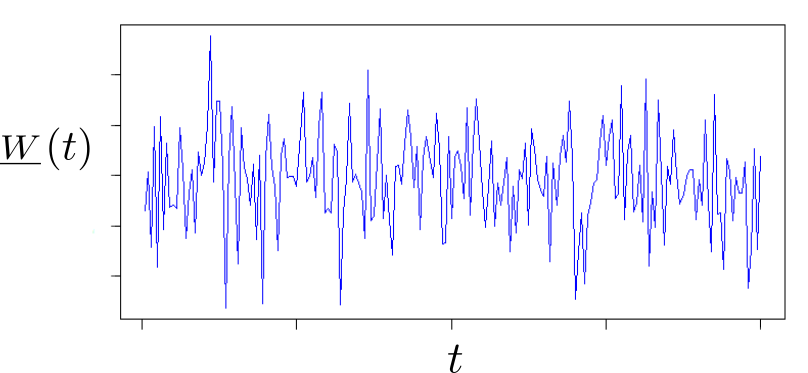
\includegraphics[width=4in]
 {stochastic-diff-eqns/white-noise-labeled}
 \caption{One dimensional white noise $\rvW(t)$}
 \label{fig-white-noise-t}
 \end{figure}
 
 \begin{figure}[h!]
  \centering
  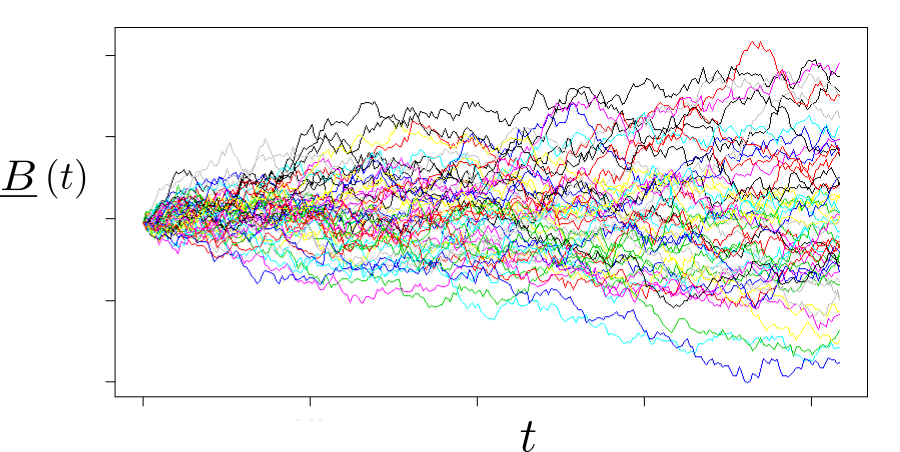
\includegraphics[width=4in]
  {stochastic-diff-eqns/brownian-motion-labeled}
  \caption{One dimensional Brownian motion $\rvB(t)$}
  \label{fig-brownian-motion-t}
  \end{figure}
  
 

{\bf White noise} $\rvW(t)
\in\RR^n$ for $t\geq 0$
is a random process with the
following properties:

\begin{itemize}
\item ==========================
\beq
\rvW(t) =\caln(W(t);\mu=0, Cov=Q)
\eeq

\item ==========================

$\rvW(t)$ and $\rvW(s)$ are independent for
$t\neq s$

\item ==========================

\beq E[\rvW(t)]=0
\eeq

\item ==========================
\beq
C_\rvW(t, s) = \av{\rvW(t), \rvW^T(s)} = Q\delta(t-s)
\eeq



\end{itemize}
{\bf Brownian motion} (a.k.a. {\bf Wiener process})
$\rvB(t)\in\RR^n$
for $t\geq 0$
is a random process with the
following properties: 

\begin{itemize}

\item==========================

\beq 
\rvB(0)=0\footnote{If wish to
consider  $\rvB(0)=\beta_0\neq 0$, replace
$\rvB$ by $\rvB-\beta_0$}
\eeq

\item ==========================

\beq
\frac{
\Delta_{t_k}^{t_{k+1}}\rvB
}{\Delta_{t_k}^{t_{k+1}}t}
\sim \caln(\mu=0, Cov=Q)
\eeq

\beq
\rvW(t_k)\sim  \caln(\mu=0, Cov=Q)
\eeq

\beq
\frac
{d \rvB}{dt} = \rvW
\eeq


\item ==========================

If $\rvB(t)\in\RR^n$ and
$[r, s]\cap [r', s']=\emptyset$, then

\beq
E[(\Delta^{s}_{r}\rvB) (\Delta^{s'}_{r'}\rvB)]=0
\label{eq-non-overlap-B}
\eeq and

\beq
E[|\Delta^{t}_{s}\rvB|^2] = n|t-s|
\label{eq-overlap-B}
\eeq

For example,
\beqa
E[\Delta_1^4\rvB \Delta_3^6\rvB]
&=&
E[(\Delta_1^3\rvB + \Delta_3^4\rvB)
(\Delta_3^4\rvB + \Delta_4^6\rvB)
]
\\
&=&
E[(\Delta_3^4\rvB)^2]
\\
&=& n |4-3|
\eeqa

Eqs.(\ref{eq-non-overlap-B}) and (\ref{eq-overlap-B}) can be written together as

\beq
E[(\Delta^{s}_{r}\rvB) (\Delta^{s'}_{r'}\rvB)]=n {\rm len}([r, s]\cap [r', s'])
\eeq

\end{itemize}


\section{SDE bnet}

In this section, we
propose a bnet for a time discretized SDE.
This bnet will be constructed by combining 
some nodes of various special types that occur frequently in bnetology.
One such special type of node that we  
have discussed already, in 
Chapter
\ref{ch-marginalizer}),
is a {\bf marginalizer node} .
Here are a few others. The TPM or structural  
equation 
associated with the node are printed in blue.
\begin{itemize}

\item {\bf diff and diff0 nodes}

The diff node is defined by 

$$\xymatrix{
\rva\ar[dr]
&&\rvb\ar[dl]
\\
&
\rvx
}
$$

\beq  \color{blue}
P(x|a, b) =\indi (x =a-b)
\eeq

\beq  \color{blue}
x =a-b
\eeq
The diff0 node is the diff node with $x=0$.
 


\item {\bf accumulator nodes}

$$
\xymatrix{
\rvx_3 \ar[d]
&\rvx_2\ar[d]
&\rvx_1\ar[d]
&\rvx_0\ar[d]
\\
\rvs_3 
&\rvs_2\ar[l]
 &\rvs_1\ar[l]
  &\rvs_0\ar[l]
}$$



\beq
\color{blue}
\begin{array}{lll}
\rvs_3 &=& \rvx_3 + \rvs_2
\\
\rvs_2 &=& \rvx_2 + \rvs_1
\\
\rvs_1 &=& \rvx_1 + \rvs_0
\\
\rvs_0&=& x_0
\end{array}
\eeq

\item {\bf incrementer nodes}

$$
\xymatrix{
\rvB_3\ar[dr] 
&& \rvB_2\ar[dl]\ar[dr]
&& \rvB_1\ar[dl]\ar[dr]
&& \rvB_0\ar[dl]
\\
&\Delta^3_2\rvB 
&&\Delta^2_1 \rvB 
&&\Delta^1_0 \rvB
&
}$$

\beq\color{blue}
\begin{array}{lll}
\Delta_2^3\rvB &=& \rvB_3 - \rvB_2
\\
\Delta_1^2\rvB &=& \rvB_2 - \rvB_1
\\
\Delta_0^1\rvB &=& \rvB_1 - \rvB_0
\end{array}
\eeq

\item {\bf de-incrementer nodes}
$$
\xymatrix{
&\Delta^3_2\rvx_2 \ar[dl] 
&&\Delta^2_1 \rvx \ar[dlll]\ar[dl]
&&\Delta \rvx^1_0 \ar[dlllll]\ar[dlll]\ar[dl]
&
\\
\rvx_3 
&& \rvx_2 
&& \rvx_1
&& \rvx_0
\ar@/^1pc/[ll]
\ar@/^1pc/[llll]
\ar@/^1pc/[llllll]
}
$$
\beq
\color{blue}
\begin{array}{lll}
\rvx_3 &=& \Delta_2^3\rvx + \Delta_1^2\rvx
+ \Delta^1_0\rvx + x_0
\\
\rvx_2 &=& \Delta_1^2\rvx
+ \Delta^1_0\rvx + x_0
\\
\rvx_1 &=&
\Delta^1_0\rvx + x_0
\\
\rvx_0&=&x_0
\end{array}
\eeq
\end{itemize}

\hrule \noindent{\bf SDE bnet}

Fig.\ref{fig-sde-3-nodes} gives a bnet for a
general one-dimensional ($n=1$) SDE defined by


\beq
d\rvx= f(\rvx, t)dt + L(\rvx, t)d\rvB(t)
\eeq
with $\rvx, \rvB\in \RR$.
Some of the structural equations, printed in blue,
for the bnet of Fig.\ref{fig-sde-3-nodes}, are
as follows.

\begin{figure}
$$
\xymatrix{
\rvB_3\ar@[red][dr] 
&& \rvB_2\ar@[red][dl]\ar@[red][dr]
&& \rvB_1\ar@[red][dl]\ar@[red][dr]
&& \rvB_0\ar@[red][dl]
\\
&\Delta^3_2\rvB \ar[d]
&&\Delta^2_1 \rvB \ar[d]
&&\Delta^1_0 \rvB \ar[d]
&
\\
&\Delta^3_2\rvx \ar@[green][dl] 
&&\Delta^2_1 \rvx \ar@[green][dlll]\ar@[green][dl]
&&\Delta^1_0\rvx \ar@[green][dlllll]\ar@[green][dlll]\ar@[green][dl]
&
\\
\rvx_3 
&& \rvx_2 \ar[lu] 
&& \rvx_1 \ar[lu]
&& \rvx_0\ar[lu]
\ar@[green]@[green]@/^1pc/[ll]
\ar@[green]@/^1pc/[llll]
\ar@[green]@/^1pc/[llllll]
}
$$
\caption{Bnet for general SDE with $N=4$ number of times. Note that this bnet
contains within it first an incrementer bnet
(in red) for the $\rvB_i$,
and
then a de-incrementer bnet (in green)
for the $\rvx_i$.}
\label{fig-sde-3-nodes}
\end{figure}




\beq
\color{blue}
\Delta_{2}^{3}\rvB = 
\rvB_3 -\rvB_2
\eeq

\beq
\color{blue}
\Delta_{2}^{3}\rvx = 
f(x_3, t)\Delta_2^3 t +
L(x_3, t)\Delta_{2}^{3}\rvB
\eeq

\beq\color{blue}
\rvx_3 = \Delta_{2}^{3}\rvx
+\Delta_{1}^{2}\rvx
+\Delta_{0}^{1}\rvx
+x_0
\eeq





\section{Simple Properties of SDE}
In this section,
we discuss several simple properties
of SDEs.

\subsection{STD with Constant Coefficients (CC)}
The most general system discussed in this 
chapter obeys the following SDE 

\beq
dx_\mu =
f_\mu(x, t)dt + L_{\mu, \nu}(x,t)d\rvB_\nu(t)
\eeq
where $\mu, \nu\in [n]$.
A system for which $f$ and $L$ are
both constant (i.e., independent of the event $(x,t)$) is said to have CC {\bf Constant Coefficients}\footnote{Ref.\cite{sar-sol},
on which most of this this chapter is
based, calls systems with CC, LTI (linear, time-invariant) systems.}


\subsection {Transition Probability Matrices}

Suppose  $t,s\geq 0$ and $x, y\in \RR^n$,
We define 
the {\bf event transition probability matrix (TPM)} as

\beq
P(\XT{y}{t}|\XT{x}{s})
\eeq

If you are familiar with the Dirac bra-ket
notation used in Quantum Mechanics,
a TPM can be expressed in such notation as 

\beq \av{y|P_{t,s}|x}\eeq
where $\{\ket{x}: x\in\RR^n\}$ is a
complete orthonormal basis:
\beq
\int dx\;\ket{x}\bra{x}
=1,\quad 
\av{y|x} = \delta(y-x)
\eeq

\subsection{Markov chain}

Let $\rvx(t_k)=x_k$ for $k\in[N]$. The bnet 
$$
x_0\rarrow\rvx_1\rarrow \rvx_2\rarrow\cdots\rarrow\rvx_{N-1}$$
is called a {\bf Markov chain}. It satisfies

\beq
P(x_{i+1}| x_i, x_{i-1}, \ldots, x_0)=
P(x_{i+1}| x_i)
\eeq
For continuous instead of discrete time,
the Markov chain definition is generalized
as follows.
For $s<t$, 
\beq
P(x(t)| x([0, s]))=
P(x(t)| x(s))
\eeq
\subsection{Chapman-Kolgomorov Equation}

\begin{claim}
(Chapman-Kolgomorov equation)

Let $x(t_k) = x_k$

\beq
P(x_3|x_1) =\int dx^n_2\; P(x_3|x_2)P(x_2|x_1)
\eeq
\end{claim}
\proof

\beqa
P(x_3, x_2|x_1) &=&
P(x_3|x_2, x_1)P(x_2|x_1)
\\
&=&
P(x_3|x_2)P(x_2|x_1)
\eeqa
Now integrate both sides over $x_2$.
\qed


\subsection{Martingale}

Let $0<t, t_i < T$ and $x(t_i)=x_i$
for $i\in[N]$.
A {\bf martingale}  for discrete (resp., continuous) time is a process $\rvy_i$ (resp., $\rvy(t)$)
which satisfies


\beq
E[\;|\rvy(t_i)|\;] < \infty\quad \forall i\quad
(\text{resp., }E[\;|\rvy(t)|\;] < \infty \quad \forall t\geq 0) 
\eeq 


\beq
E\left[\rvy(t)|x(t_{[i\upto j]})\right]= y(t_j)
\quad (\text{resp., }E\left[\rvy(t)|x([0,s])\right]= y(s))
\eeq


Brownian motion is a martingale.
\beq
E[\rvB(t)| B(t_{[i\upto j]}] = B(t_j)
\eeq


It\^{o} integrals $\int L\XT{x}{t}d\rvB_t$ (discussed later)
are martingales too, but Stratonovich integrals (discussed later)
$\int L\XT{x}{t}\circ d\rvB_t$
aren't. 





\section{It\^{o} Integral}

Consider the 1 dimensional case $\rvx, \rvW\in \RR$.
\beq
\frac{d\rvx}{dt}= f(\rvx, t) + L(\rvx, t)\rvW(t)
\eeq

\beq
\rvx(t) - \rvx(0) =
\int_{0}^{t}dt\; f(x,t) + J
\eeq
where

\beq
J = \int_{0}^t dt\;
L(x, t)\rvW(t)
\eeq

For $t_0=0 < t_1 <\ldots <t_{N-1}$, $t_k^*\in [t_k, t_{k+1})$, define



\beq 
J_N = 
\sum_k L(\rvx, t_k^*)\Delta_{t_k}^{t_{k+1}}\rvB
\eeq
and

\beq 
J = \lim_{N\rarrow \infty} J_N
\eeq

$L(x,t)\rvW(t)$ is called an integrand,
In non-rigorous calculus,
we normally consider integrands
that are smooth, so that as $N\rarrow \infty$
and the separation between successive $t_i$
goes to zero,
the value of $J$
is independent of where $t^*_k$
is located inside the interval $[t_k, t_{k+1})$.
In the SDE case, the integrand $L\rvW$ is continuous
but very jagged, so the value of $J$ does
depend on the choice of $t^*_k$.

Consider the special case that
$L=\rvx=\rvB$, so 

\beq
J_N=\sum_k \rvB(t_k^*) \Delta_{t_k}^{t_{k+1}}\rvB
\eeq
Let us see how in this simple case,
the value of $J$ depends on the
choice of $t^*_k$.

\begin{enumerate}

\hrule
\item $t_k^* = t_{k+1}$ 
\beqa
E[J_N] &=&
\sum_k E[\rvB(t_{k+1})\Delta_{t_k}^{t_{k+1}}\rvB] 
\\
&=&
\sum_k
E[(\Delta_{0}^{t_{k+1}}\rvB)\Delta_{t_k}^{t_{k+1}}\rvB] 
\\
&=&
\sum_k
E[(\Delta_{t_k}^{t_{k+1}}\rvB)^2]
\\
&=&t
\eeqa

\hrule
\item $t_k^* = \frac{t_k + t_{k+1}}{2}$
Stratonovich integral

\hrule
\item $t_k^* = t_k$, Ito integral\footnote{More correctly,
It\^{o}}


\beqa
E[J_N] &=&\sum_k E[\rvB(t_k)\Delta_{t_k}^{t_{k+1}}\rvB] 
\\
&=& \sum_k
E[(\Delta_{0}^{t_k}\rvB)\Delta_{t_k}^{t_{k+1}}\rvB] 
\\
&=&0
\eeqa

\beqa
J_N &=& 
\sum_k \rvB(t_k)\Delta_{t_k}^{t_{k+1}}\rvB
\\
&=&
\frac{1}{2}\sum_k\left[
-[\Delta_{t_k}^{t_{k+1}}\rvB]^2
+ \Delta_{t_k}^{t_{k+1}}(\rvB^2)\right]
\eeqa

\beqa
J &=& \lim_{N\rarrow \infty} J_N
\\
&=&
\frac{1}{2}
(-t+\rvB^2(t))
\eeqa
$E[J] = \frac{1}{2}(-t+t)=0$






\end{enumerate}

\beq
d[\rvB^2(t)]=
2\rvB(t)d\rvB(t)
+t
\eeq


\beq
[d\rvB(t)]^2 = dt
\eeq



For $\rvB\in\RR^n$,

\beq
\boxed{
d[\rvB_\alpha(t)\rvB_\beta(t)]=\delta(\alpha, \beta)
\left[
2\rvB_\alpha(t)d\rvB_\alpha(t)
+nt\right]}
\eeq

\beq
\boxed{
d[\rvB_\alpha(t)]d[\rvB_\beta(t)]
=Q_{\alpha, \beta}dt}
\eeq






\section{Fokker-Planck Equation}


Consider the $n$ dimensional case $\rvx, \rvW\in \RR^n$. Let $\mu, \nu,\alpha, \beta\in [n]$. Suppose
\beq
d\rvx_\mu= f(\rvx, t)dt + L(\rvx, t)d\rvB_\mu(t)
\eeq
where

\beq
R_{\mu, \nu} = \frac{1}{2} L_{\mu,\alpha}Q_{\alpha,\beta}L^T_{\beta,\nu}
\eeq


\begin{claim}
\beq
d\phi=
\left[\pder{\phi}{t} +
 f_\mu\pder{\phi}{x_\mu} + 
 R_{\mu, \nu}
\frac{\partial^2\phi}{\partial x_\mu\partial x_\nu}\right]dt
+
\pder{\phi}{x_\mu}L_{\mu,\nu}d\rvB_\nu
\eeq
\end{claim}
\proof

The Taylor
expansion of $\phi(x,t)$, up to second
order derivatives, is

\beq
d\phi =
\pder{\phi}{t}dt
+
\sum_\mu \pder{\phi}{x_\mu} d\rvx_\mu
+\frac{1}{2}
\sum_\mu \sum_\nu \frac{\partial^2\phi}{\partial x_\mu\partial x_\nu}d\rvx_\mu d\rvx_\nu
\eeq


\beq
\pder{\phi}{x_\mu} d\rvx_\mu
=
\pder{\phi}{x_\mu} 
\left[
f_\mu dt + L_{\mu, \nu}d\rvB_\nu
\right]
\eeq

\beqa
\frac{\partial^2\phi}{\partial x_\mu\partial x_\nu}d\rvx_\mu d\rvx_\nu
&=&\frac{\partial^2\phi}{\partial x_\mu\partial x_\nu}
\left[
f_\mu dt + L_{\mu, \alpha}d\rvB_\alpha
\right]
\left[
f_\nu dt + L_{\nu, \beta}d\rvB_\beta
\right]
\\
&=&
\frac{\partial^2\phi}{\partial x_\mu\partial x_\nu}
L_{\mu, \alpha}  L_{\nu, \beta} d\rvB_\alpha d\rvB_\beta
\\
&=&
\frac{\partial^2\phi}{\partial x_\mu\partial x_\nu}
L_{\mu, \alpha}  L_{\nu, \beta} Q_{\alpha,\beta} dt
\eeqa

\beqa
d\phi &=&
\pder{\phi}{t}dt
+
\pder{\phi}{x_\mu} [f_\mu dt + L_{\mu,\nu}d\rvB_\nu]
+ R_{\mu, \nu}
\frac{\partial^2\phi}{\partial x_\mu\partial x_\nu}dt
\\
&=&
\left[\pder{\phi}{t} +
f_\mu \pder{\phi}{x_\mu} + R_{\mu, \nu}
\frac{\partial^2\phi}{\partial x_\mu\partial x_\nu}\right]dt
+
\pder{\phi}{x_\mu}L_{\mu,\nu}d\rvB_\nu
\eeqa

\qed

For example,  if $n=1$, $\rvx=\rvB$, 
$\phi = \rvB^K$
and
$L=Q=1$, $f=0$,
we get

\beq
d(\rvB^m) = \left[m \rvB^{m-1}+ m(m-1) \rvB^{m-2}\right]dt
+ m\rvB^{m-1}d\rvB
\eeq

The next claim defines the {\bf Fokker-Planck equation} (FP equation) (a.k.a. {\bf Fokker-Planck-Kolgomorov equation} )
for the probability $P(x,t)$
of single event $(x,t)$


\begin{claim} 
(Forward FP equation)

Assume
\beq
dx = f(x, t)dt + L(x, t)d\rvB
\eeq
Then

\beq
	\pder{P(x, t)}{t}= \calf_\rvx P(x, t)
	\eeq
with

\beq
\calf_\rvx \bullet=
-\;\pder{}{x_\mu}
(\bullet f_\mu) + 
\frac{\partial^2}{ \partial x_\mu\partial x_\nu}(\bullet R_{\mu, \nu})
\eeq
\end{claim}
\proof

\beq
\int dx^n\; P\XT{x}{t}\left[ \pder{\phi}{x_\mu}L_{\mu,\nu}d\rvB_\nu
\right]
=0
\eeq

Integration by parts

\beq
udv = d(uv)-(du)v 
\eeq

\beq
\int_{-\infty}^{+\infty}udv=
\underbrace{uv|_{-\infty}^{+\infty}}_{0}
\quad
-
\int_{-\infty}^{+\infty}(du)v 
\eeq



\beq
\int dt dx^n\; P\XT{x}{t}\frac{d\phi}{dt}=
\int dt dx^n\; P\XT{x}{t}
\left[\pder{\phi}{t} +
 f_\mu\pder{\phi}{x_\mu} + R_{\mu, \nu}
\frac{\partial^2\phi}{\partial x_\mu\partial x_\nu}\right]
\eeq



\beq
-\int dt dx^n\; \phi\frac{dP}{dt}=
\int dt dx^n\;  \phi
\left[-\;\pder{P}{t} -
\pder{(Pf_\mu)}{x_\mu} + 
\frac{\partial^2 }{\partial x_\mu\partial x_\nu}(PR_{\mu, \nu})\right]
\eeq
\qed

\begin{claim}
	\beq
	\pder{P}{t}= \calf_\rvx P
	\eeq
	is solved formally by
	
	\beq
	P(x,t)=e^{(t-t_0)\calf_\rvx}P(x, t_0)
	\eeq
\end{claim}
\proof
Just use the Taylor expansion of an exponential function and analogize with the case when $\calf_\rvx$ is a constant.
\qed

Note that 
\beq
\pder{P}{t} = -\pder{J_\mu}{x_\mu}
\label{eq-cons-prob}
\eeq
where

\beq
J_\mu = Pf_\mu - \pder{(PR_{\mu,\nu})}{x_\nu}
\eeq

Eq.(\ref{eq-cons-prob})
is the {\bf equation for conservation of probability}\footnote{It implies conservation of probability because
$$0=\pder{}{t}\int_V dV\;P=
\int_V dV\;\nabla\cdot \vec{J}= 
\int \vec{J}\cdot d\vec{S}$$
}. $J_\mu$ is called the {\bf probability
flux}, $f_\mu$ is called the {\bf drift},
and $R_{\mu, \nu}$ is called the
{\bf diffusion matrix} (or {\bf diffusion coefficient} if it's a scalar)

The forward FP equation when  $n=1$, $f=0$, $L=1$, $R=D>0$, is called the {\bf Diffusion Equation}.

\beq
dx = d\rvB
\eeq

\beq
\pder{P}{t} = D
\frac{\partial^2P}{\partial^2x}
\eeq

As another example of the forward FP,
consider the
{\bf Overdamped Langevin Equation}\footnote{
This equation, also known as Brownian dynamics (see
Ref.\cite{wiki-brownian-dyn}),  arises from
Newton's equation $m\ddot{x}= -\lam\dot{x}  -U'(x)$ when the acceleration $\ddot{x}$ is negligible, so the drag force and potential force cancel each other.} 

\beq
dx_\mu = -\;\frac{1}{2}\pder{U}{x_\mu}dt + d\rvB
\eeq

\begin{claim}
For the overdamped Langevin equation,
if $Q =\frac{1}{\lam}>0$, then the steady state 
solution is

\beq
P(x) = \frac{e^{-\lam U(x)}}{Z}
\eeq
where 
\beq
Z = \int dx^n\;e^{-\lam U(x)}
 \eeq

\end{claim}
\proof

The forward FP equation with
$L=1$, $\pder{P}{t}=0$ is
\beq
0= -
\pder{(Pf_\mu)}{x_\mu} + \frac{1}{2\lam}
\frac{\partial^2 P }{\partial x_\mu^2}
\eeq
If we substitute $f_\mu =-\; \frac{1}{2}\pder{U}{x_\mu}$ into this, we get


\beq
0= \frac{1}{2}
\pder{}{x_\mu}\left(P\pder{U}{x_\mu} + \frac{1}{\lam}
\pder{P }{x_\mu}
\right)
\eeq
If we now substitute the proposed value of $P$, we get $0=0$

\beq
0=
\pder{}{x_\mu}\left(\lam e^{-\lam U}\pder{U}{x_\mu}+
\pder{e^{-\lam U}}{x_\mu}
\right) 
\eeq

\qed

Recall

\beq
\calf_\rvx \bullet=
-\;\pder{}{x_\mu}
(\bullet f_\mu) + 
\frac{\partial^2}{ \partial x_\nu\partial x_\mu}(\bullet R_{\mu, \nu})
\eeq

Define $\calb_\rvx$ to be the same as $\calf_\rvx$
but with every derivative $A\pder{B}{x_\mu}$
replaced by $-B\pder{A}{x_\mu}$. Hence\footnote{For those
	who know Quantum Mechanics, our $\calf$ equals 
	a Hamiltonian $H$ times $i$, $\calf =Hi$.
}

\beq
\calb_\rvx \bullet=
f_\mu\pder{\bullet}{x_\mu}
 + R_{\mu, \nu}
\frac{\partial^2\bullet}{\partial x_\mu\partial x_\nu}
\eeq



\begin{claim} (Forward FP equation for transition matrix $ P(\XT{x}{t}|\XT{w}{s})$)

$ P(\XT{x}{t}|\XT{w}{s})$ satisfies
	
\beq
\pder{P(\XT{x}{t}|\XT{w}{s})}{t}=
\calf_\rvx P(\XT{x}{t}|\XT{w}{s})
\label{eq-forward-fp-tm}
\eeq
with
\beq
P(\XT{x}{s}|\XT{w}{s})=\delta(x-w)
\eeq

In case you know Dirac bra-ket notation, the 
differential
equation Eq.(\ref{eq-forward-fp-tm})
 can be expressed in Dirac notation as

\beq
\pder{\av{x|P_{t,s}|w}}{t}
=\int 
\av{x|\calf_{t}|x'}dx'\av{x'|P_{t,s}|w}
\eeq
with

\beq
\av{x|P_{s,s}|w} =\delta(x-w)
\quad \text{(Hence, $P_{s,s}=1$)}
\eeq
\end{claim}


	
	
\begin{claim} (Backward FP equation for transition matrix $P(\XT{y}{u}|\XT{x}{t})$)

$P(\XT{y}{u}|\XT{x}{t})$ satisfies
\beq
-\;\pder{P(\XT{y}{u}|\XT{x}{t})}{t}=
\calb_\rvx P(\XT{y}{u}|\XT{x}{t})
\label{eq-backward-fp-tm}
\eeq
with

\beq
P(\XT{y}{t}|\XT{x}{t}) =\delta(y-x)
\eeq

In case you know Dirac bra-ket notation, the 
differential
equation Eq.(\ref{eq-backward-fp-tm})
 can be expressed in Dirac notation as

\beq
-\; \pder{\av{y|P_{u,t}|x}}{t}
=\int 
\av{y|\calb_t|y'}dy'\av{y'|P_{u,t}|x}
\eeq
with
\beq
\av{y|P_{t,t}|x}=\delta(y-x)
\quad \text{(Hence, $P_{t,t}=1$)}
\eeq
	
\end{claim}

The forward FP equation is the
time reversed version of the 
backward FP equation. Thus, they describe 
the same stochastic process,
in opposite time directions.

Note that if we view
a transition matrix 
$P(\XT{y}{u}|\XT{x}{t})$  as a matrix whose rows and columns are labeled by 
all possible events $(\XT{x}{t})$, then the forward FP equation (resp., backward FP equation)
is a differential equation
constraining all the rows $(\XT{y}{u})$ for a fixed column
$(\XT{x}{t})$
(resp., all the columns for a fixed row).
They both constrain
the same matrix $P(\XT{y}{u}|\XT{x}{t})$,
but in 2 different ways.

	






\section{First and second order statistics}
In this section,
we derive differential equations
for the  first and second order statistics
of an SDE without and with CC.
\subsection{For general SDE}
Suppose the SDE coefficients $f$ and $L$
can depend on the event $(x,t)$.


Let
\beq
m_\mu(t) = E[\rvx_\mu(t)]=
\av{\rvx_\mu(t)}
\eeq

\beq
C_{\mu, \nu}(t,s) = \av{\rvx_\mu(t), \rvx_\nu(s)}
\eeq

\beq
V_{\mu, \nu}(t) = C_{\mu, \nu}(t,t)
\eeq


\beq
dx_\mu = \left[a_\mu(t) + F_{\mu, \nu}(t)x_\nu \right] dt + 
L_{\mu, \nu}(t)d\rvB_\nu
\eeq

\beq
R_{\mu, \nu} = 
\frac{1}{2}L_{\mu, \alp}Q_{\alp, \beta}L^T_{\beta, \nu} =\frac{1}{2} (LQL^T)_{\mu, \nu}
\eeq

\begin{claim}
\label{cl-mt-Vt}
\beq
\frac{dm}{dt}=
a + Fm
\eeq

\beq
\frac{dV}{dt}=
VF^T +FV^T+ 2R
\eeq

\end{claim}
\proof

\beqa
\frac{dm}{dt}&=&
\av{a + F\rvx}
\\\
&=&
a + Fm
\eeqa

Let $\partial_\alp =\pder{}{x_\alp}$
\beqa
d\av{\rvx_\mu, \rvx_\nu}
&=&
dx_\alp\partial_\alp\av{\rvx_\mu, \rvx_\nu}
+
dx_\alp dx_\beta\frac{1}{2}\partial_\alp\partial_\beta\av{\rvx_\mu, \rvx_\nu}
\\
&=&
\av{\rvx_\mu, 
d\rvx_\nu}
+
\av{d\rvx_\mu, 
\rvx_\nu}
+ \av{d\rvx_\mu, d\rvx_\nu}
\\
&=&
\av{\rvx_\mu, 
F_{\nu,\alp}\rvx_\alp dt}
+
\av{F_{\mu,\alp}\rvx_\alp dt, 
\rvx_\nu}
+ 
2R_{\mu, \nu}dt
\\
&=&
(VF^T+FV^T+2R)dt
\eeqa
\qed

We call a {\bf propagator}, a function $\Psi:\RR^+\times \RR^+\rarrow \RR$
that satisfies
\beq
\pder{\Psi(t, s)}{t}  = F(t) \Psi(t, s)
\eeq

\beq
\begin{array}{l}
\Psi(a, c) = \Psi(a, b)\Psi(b, c)
\\
\Psi^{-1}(a,b) = \Psi(b,a)
\\
\Psi(a,a)=1
\end{array}
\eeq



\begin{claim}
\beq
m(t) = \Psi(t, t_0)m(t_0) +\int_{t_0}^{t}d\tau\;
\Psi(t, \tau)a(t)
\label{eq-mt-psi}
\eeq

\beq
V(t)=\av{\rvx(t), \rvx^T(t)}=\Psi(t, t_0)V(t_0)\Psi^T(t, t_0)
+
\int_{t_0}^t d\tau\; \Psi(t, \tau)R(\tau)
\Psi^T(t, \tau)
\label{eq-Vt-psi}
\eeq


\beq
\av{\rvx(t), \rvx^T(s)} = 
\left\{
\begin{array}{ll}
V(t)\Psi^T(s,t) &\text{if } t<s
\\
\Psi(t,s)V(s) & \text{if }t\geq s
\end{array}
\right.
\label{eq-sde-cov-s-t}
\eeq
\end{claim}
\proof
Eqs.(\ref{eq-mt-psi} and (\ref{eq-Vt-psi}))
can be proven simply by taking the time derivative of both sides.
This yields the differential
equations for $m(t)$ and $V(t)$ that were established in Claim \ref{cl-mt-Vt}.
We won't prove Eq.(\ref{eq-sde-cov-s-t}) here.
For a proof,  see
Ref.\cite{sde-applied-book}.
\qed



If $P(x,t=0)$ is a Gaussian, $P(x,t)$ must be Gaussian too,
because the transformation is linear. Therefore,

\beq
P(x,t) = P(x(t))=
\caln(x(t); \mu=m(t), \Sigma^2=V(t))
\eeq

\beq
P(x(t)|x(s)) =\caln(x(t); \mu=m(t|s), \Sigma^2=V(t|s))
\eeq
where

\beq
m(t|s) =
\Psi(t,s)x(s)
+\int_{t_0}^t d\tau \Psi(t, \tau)a(\tau)
\eeq

\beq
V(t|s)=\int_s^td\tau\;
\Psi(t, \tau)
R(\tau)\Psi^T(t, \tau)
\eeq

This transition matrix $P(x(t)|x(s))$, when we discretize time and set $x(t_k)=x_k$, defines the 
dynamic bnet of Fig.\ref{fig-1st-2nd-order-bnet}.
Define

\beq 
\Psi_k = \Psi(t_{k+1}, t_k)
\eeq

\beq
a_k = \int_{t_k}^{t_{k+1}}
d\tau\; \Psi(t_{k+1}, \tau)a(\tau)
\eeq

\beq
\Sigma_k=
\int_{t_k}^{t_{k+1}}d\tau\;
\Psi(t_{k+1}, \tau)R(\tau)\Psi^T(t_{k+1}, \tau)
\eeq
The TPMs,
printed in blue, for the bnet of Fig.\ref{fig-1st-2nd-order-bnet}, are as follows:

\beq \color{blue}
P(x_{k+1}|x_k)= \indi(x_{k+1}=\Psi_kx_k + a_k +\eps_k)
\eeq

\beq \color{blue}
P(\eps_k) = \caln(\eps_k; \mu=0, \Sigma=\Sigma_k)
\eeq




\begin{figure}[h!]
$$
\xymatrix{
\ul{\eps}_3 \ar[d]
& \ul{\eps}_2 \ar[d]
& \ul{\eps}_1 \ar[d]
& \ul{\eps}_0\ar[d]
\\
\rvx_3 
& \rvx _2 \ar[l]
& \rvx_1 \ar[l]
& \rvx_0\ar[l]
}
$$
\caption{Bnet that satisfies the general SDE, 
assuming $P(x,t=0)$ is a Gaussian.}
\label{fig-1st-2nd-order-bnet}
\end{figure}





\subsection{In case SDE has CC}
When the SDE has CC,
\beq
\Psi(t, s) = e^{(t-s)F}
\eeq


At time $t=\infty$, 
a system with CC reaches
a {\bf steady state} (i.e., zero time derivatives of expected values)
with mean value $m_\infty$
and variance $V_\infty$ given by
\beq
0=a + Fm_\infty
\eeq
\beq
0=V_\infty F^T  + F v_\infty^T + 2R 
\eeq


\section{Fourier Analysis for CC case}

In this section, we will apply Fourier
analysis to the SDE with CC.

We begin by recalling a few definitions from Fourier 
analysis.

\newcommand{\Tintegral}[1]{
\int_{-\;\frac{T}{#1}}^{\frac{T}{#1}}}

The Dirac delta function satisfies:

\beq
\delta(t) =\frac{1}{2\pi} \int_{-\infty}^{\infty}d\omega \;e^{i\omega t}
\eeq
The Fourier Transform of $x(t)$ is
\beq
\TIL{x}(\omega)=\calf[x(t)](\omega)=
\int_{-\infty}^{\infty}dt\; x(t) e^{-i\omega t}
\eeq
The inverse Fourier transform of $\TIL{x}(\omega)$ is
\beq
x(t)=\calf^{-1}[x(\omega)](t)=
\frac{1}{2\pi}
\int_{-\infty}^{\infty}d\omega\; \TIL{x}(\omega) e^{i\omega t}
\eeq

\beq
x_T(\omega)=\Tintegral{2}
dt\;x(t) e^{-i\omega t}
\eeq


Define the 
{\bf power spectral density}
of process $x(t)$ is by
\beq
S_\rvx(\omega)= \lim_{T\rarrow 0}
\frac{1}{T} E[\TIL{x}_T(\omega)\TIL{x}^\dagger_T(\omega)]
\eeq
In case $\rvx=\rvW$= white noise,


\beq 
S_{\rvW}(\omega) = Q
\eeq

Define the
{\bf autocorrelation function for stationary process $\rvx(t)$} by
\beq
AC_\rvx(\tau)=
E[x(t)x^T(t+\tau)]
\eeq
$\tau$ is called the {\bf time lag}.

\begin{claim}


\beq 
\Tintegral{2}dt
\Tintegral{2}ds\;
g(t-s)=
\int_{-T}^{T}d\tau\;g(\tau)(T-|\tau|)
\label{eq-ac-integral-formula}
\eeq
\end{claim}
\proof

Let 

\beq 
\tau=\frac{t-s}{\sqrt{2}},\quad
\sigma=\frac{t+s}{\sqrt{2}}
\eeq
The absolute value of the Jacobian $|\frac{\partial(s, t)}{\partial(\tau, \sigma)}|$ equals 1.
Hence,

\begin{align}
\Tintegral{2}dt
\Tintegral{2}ds\;
g(t-s)
&=
\Tintegral{\sqrt{2}}d\tau
\int_{-\;\frac{T}{\sqrt{2}}-|\tau|}
^{\frac{T}{\sqrt{2}}+|\tau|}d\sigma \;g(\sqrt{2}\tau)
\quad(\text{See Fig. \ref{fig-integral-region}})
\\
&=
\Tintegral{\sqrt{2}}d\tau
\;g(\sqrt{2}\tau)
(\sqrt{2}T - 2|\tau|)
\\
&=
\int_{-T}
^{T}d\tau'
\;g(\tau')
(T - |\tau'|)\quad(\tau' = \sqrt{2}\tau)
\end{align}

\begin{figure}[h!]
\centering
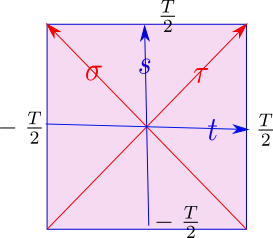
\includegraphics[width=1.5in]
{stochastic-diff-eqns/integral.png}
\caption{Integration
region
for integral given by Eq.(\ref{eq-ac-integral-formula})}
\label{fig-integral-region}
\end{figure}


\qed

\begin{claim}(Wiener Khinchin theorem (WK))

\beq
S_\rvx(\omega)
=
\int_{-\infty}^{\infty}d\tau\; AC_\rvx(\tau)e^{-i\omega \tau}
\eeq
If $AC(\tau)=AC(-\tau)$,

\beq
S_\rvx(\omega)
=
2\int_{0}^{\infty}d\tau\; AC_\rvx(\tau)\cos(\omega\tau)
\eeq

\end{claim}
\proof

\begin{align}
\int_{-\infty}^{\infty}d\tau\;
AC_\rvx(\tau)
e^{-i\omega\tau}
&=
\int_{-\infty}^{\infty}d\tau\;
\av{x(t)x^\dagger(t+\tau)}
e^{-i\omega\tau}
\\
&=
\int_{-\infty}^{\infty}d\tau
\int_{-\infty}^{\infty}\frac{d\omega_1}{2\pi}
\int_{-\infty}^{\infty}\frac{d\omega_2}{2\pi}
\av{\TIL{x}(\omega_1)\TIL{x}^\dagger(\omega_2)}
e^{-i\omega\tau+i\omega_1t-i\omega_2(t+\tau)}
\end{align}

To get rid of the $t$ dependence on the right hand side
of the last equation, apply $\frac{1}{T}\int_{-T/2}^{T/2}$ to both sides
to get


\begin{align}
\int_{-\infty}^{\infty}d\tau\;
AC_\rvx(\tau)
e^{-i\omega\tau}
&=
\int_{-\infty}^{\infty}\frac{d\tau}{T}
\int_{-\infty}^{\infty}\frac{d\omega_1}{2\pi}
\int_{-\infty}^{\infty}d\omega_2
\av{\TIL{x}(\omega_1)\TIL{x}^\dagger(\omega_1)}
e^{-i(\omega+\omega_2)\tau}
\delta(\omega_1-\omega_2)
\\
&=
\int_{-\infty}^{\infty}\frac{d\tau}{T}
\int_{-\infty}^{\infty}\frac{d\omega_1}{2\pi}
\av{\TIL{x}(\omega_1)\TIL{x}^\dagger(\omega_1)}
e^{-i(\omega+\omega_1)\tau}
\\
&=
\frac{1}{T}
\int_{-\infty}^{\infty}d\omega_1
\av{\TIL{x}(\omega_1)\TIL{x}^\dagger(\omega_1)}
\delta(\omega+\omega_1)
\\
&=
\frac{1}{T}
\av{\TIL{x}(\omega)\TIL{x}^\dagger(-\omega)}=
\frac{1}{T}
\av{\TIL{x}(\omega)\TIL{x}^T(\omega)}
\end{align}
Alternative proof:


\beqa
\frac{1}{T}
E[|\TIL{x}_T(\omega)|^2]
&=&\frac{1}{T}
\Tintegral{2}ds
\Tintegral{2}dt\; 
E[x(t)x^T(s)]e^{-iw(t-s)}
\\
&=&\frac{1}{T}
\int_{-T}^{T}d\tau\;
AC(\tau)e^{-i\omega \tau}(T-|\tau|)
\\
&\rarrow&
\int_{-\infty}^{\infty}d\tau\; AC(\tau)e^{-i\omega \tau}
\quad\text{(Use Eq.(\ref{eq-ac-integral-formula}))}
\eeqa
\qed

As a trivial example of the WK theorem, note that
\beq
AC_{\rvW}(\tau) = Q\delta(\tau)
\eeq
Hence,  by the WK theorem,

\beq
S_\rvx(\omega)=Q
\eeq

Next, let us solve the 
SDE with CC using Fourier Transforms. 
Substituting Fourier Transforms for $x(t)$
into this equation we get 
\beq
\frac{d x}{dt}=Fx + L\rvW
\eeq
we get

\beq
-i\omega \TIL{x} = F\TIL{x} + L\TIL{\rvW}
\eeq
Hence,

\beq
\TIL{x}= -( F+i\omega)^{-1}L\TIL{\rvW}
\eeq

\beqa
S_{\rvW}(\omega) &=& \TIL{x}\TIL{x}^\dagger
\\
&=&
(F+i\omega)^{-1}\underbrace{LQL^\dagger}
_{2R}(F^T-i\omega)^{-1}
\eeqa

\beq
AC_{\rvx}(\tau)= 
\int_{-\infty}^{\infty}d\omega\; e^{-i\omega \tau}
(F+i\omega)^{-1}(2R)
(F^T-i\omega)^{-1}
\eeq

When steady state is reached,
the expected values (averages) of functions of $\rvx(t)$ cease to vary with time. Thus, we only need to compare $\rvx(t)$
to itself, not to $\rvx(t+\tau)$ with $\tau>0$. 
Hence, we only need to know $AC(\tau)$ at $\tau=0$.


For steady state, by the Wiener Khinchin theorem, 
\beq
S_\rvx(\omega)=AC_\rvx(0) 2\pi\delta(w)
\eeq
where

\beq
AC_\rvx(0)=
\int_{-\infty}^\infty
dw\;(F+i\omega)^{-1}(2R)
(F^T-i\omega)^{-1}
\eeq


\section{Lamperti Transformation}

The {\bf Lamperti Transformation} answers
the following question: If the next two
SDE are satisfied, express $g_\mu$ in terms of $f_\mu$ and $L_{\mu, \nu}$
\beq
dx_\mu = f_\mu(x,t)dt + L_{\mu,\nu}(x,t)d\rvB_\nu
\eeq

\beq
dy_\mu = g_\mu(y,t)dt + d\rvB_\mu
\label{eq-g-def-grisa}
\eeq



\begin{claim} For $n=1$, the function 
$g(y,t)$ in Eq.(\ref{eq-g-def-grisa}) 
is given by

\beq
g(y,t)=
\left.\left(
\pder{}{t}
\int_\xi^x \frac{du}{L\XT{u}{t}}
+
\frac{f\XT{x}{t}}{L\XT{x}{t}}
-\;
\frac{1}{2}
\pder{L\XT{x}{t}}{x}
\right)\right|_{x\rarrow h^{-1}(y,t)}
\eeq
\end{claim}
\proof
Suppose
\beq
y=h\eqdef\int_\xi^x\frac{du}{L(u,t)}
\eeq
Then

\beqa
dy &=& \pder{h}{t}dt + \frac{dx}{L}
-\;\frac{1}{2L^2}
\pder{L}{x}(dx)^2
\\
&=&
 \pder{h}{t}dt + \frac{fdt +  Ld\rvB}{L}
-\;\frac{1}{2L^2}
\pder{L}{x}\underbrace{(Ld\rvB)^2}_{L^2dt}
\\
&=&
\left(
\pder{h}{t} + \frac{f}{L} -\frac{1}{2}\pder{L}{x}
\right)dt + d\rvB
\eeqa
\qed





\section{Feynman-Kac Path Integrals}

{\bf Kac path integrals} (Kac PI)
are weighted sums  over paths. Kac FPs
are solutions of a classical SDE for specific boundary conditions. They were first proposed by Kac.

{\bf Feynman path integrals} (Feynman PI) are similar to Kac PI,
but the weights of the sum are complex valued instead of real valued. Feynman FPs
are solutions of a quantum SDE (i.e., a Schroedinger equation) for specific boundary conditions.They
were first proposed by Feynman,
who  wrote a whole book
about them (see Ref.\cite{feynman-hibbs})

Despite its name,
this section will
deal only with  Kac PI.
Furthermore, we will only
consider the
the one dimensional case $\rvx\in\RR$.
The higher dimensional case
is similar.


\begin{figure}[h!]
$$
\xymatrix{
\ul{\Delta B}_3 \ar[d]
& \ul{\Delta B}_2 \ar[d]
& \ul{\Delta B}_1 \ar[d]
& \ul{\Delta B}_0\ar[d]
\\
\rvx_3 
& \rvx _2 \ar[l]
& \rvx_1 \ar[l]
& \rvx_0\ar[l]
}
$$
\caption{Bnet for defining 1-dim Kac PI.}
\label{fig-1dim-kac-pi}
\end{figure}

Let $x(t_k)=x_k$ and consider the bnet
of Fig.\ref{fig-1dim-kac-pi}.
The
TPMs, printed in blue, 
for that bnet, are as follows

\beq\color{blue}
P(x_k|x_{k+1})= \indi(x_{k-1}
+f_k\Delta t +\Delta\rvB_k)
\eeq

\beq \color{blue}
\Delta\rvB_k \sim \caln(\mu=0, \s^2=q\Delta t)
\eeq
Then

\begin{align}
P(x_{[1\upto N]})&=
\prod_{k=1}^N P(x_k|x_{k-1})
\\
&=
\prod_{k=1}^N
\left[
\frac{1}{\sqrt{2\pi q\Delta t}}
\exp\left(
-\;
\frac{(x_k-x_{k-1})^2}{2q\Delta t}
\right)
\right]
\\
&=
\prod_{k=1}^N
\left[
\frac{1}{\sqrt{2\pi q \Delta t}}
\exp\left(
-\;
\frac{(f_k\Delta t + \Delta B_k)^2}{2q\Delta t}
\right)
\right]
\\
&=
\underbrace{\prod_{k=1}^N
\left[
\frac{1}{\sqrt{2\pi q \Delta t}}
\right]}_{\gamma^N}
\exp\left(
-\;
\frac{1}
{2q}\int_0^{t_N}dt
\left[(\ddot{B})^2 +
2f\dot{B} +f^2\right]
\right)
\end{align}



\beq
P(B_{[0 \upto N]})
=
\gamma^N\exp\left(-\;
\frac{1}{2 q}\int_0^{t_N} dt (\ddot{B})^2
\right)
\eeq

\beq
\frac{P(x_{[1\upto N]})}{P(B_{[1\upto N]})}=
\exp\left(-\;
\frac{1}{2q}\int_0^{t_N}dt
\left[
2f\dot{B} +f^2\right]
\right)
\label{eq-px-div-pb}
\eeq

\beq
\cald B = \gamma^N \prod_{k=1}^N dB_k
\eeq

Note that
$(B_k, t_k)\in \RR^n\times [0, T]$
for $k\in[0-N]$.
Let
$\cale\subset \RR^n\times [0, T]$. 
Fig.\ref{fig-possible-paths}
shows a possible set $\cale$
when $n=1$.
The path integration is over all
paths $(B_k, t_k)$ for $k\in [0-N]$
that live inside $\cale$.

It follows that
\beq
P(x_{N+1}|x_0=0)  =
\int_{\cale}\cald B\;
\exp\left(
\frac{1}
{2q}\int_0^{t_N}dt
\left[(\ddot{B})^2 +
2f\dot{B} -f^2\right]
\right)
\eeq


\begin{figure}[h!]
\centering
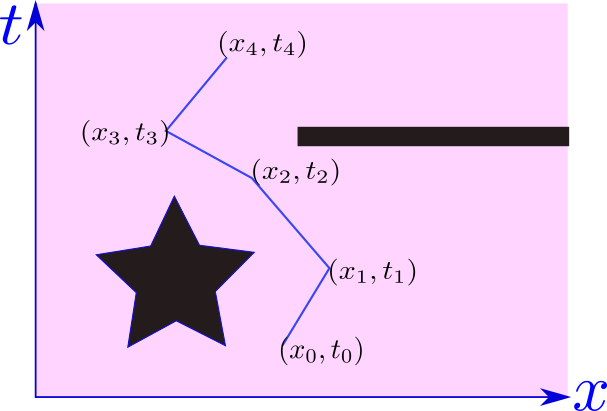
\includegraphics[width=3.5in]
{stochastic-diff-eqns/possible-paths.png}
\caption{The pink area is a possible set 
$\cale\subset\RR\times [0,T]$
such that  $(B_k, t_k)\in \cale$
}
\label{fig-possible-paths}
\end{figure}

\section{Karhunen–Loève series}

In this section
we explain the {\bf Karhunen–Loève (KL) series}. The most intuitive
way of explaining  KL series is
using Dirac bra-ket notation.

Let $\{\ket{t}
 : t\in [0,T]\}$ be a complete orthonormal basis
\beq
\int_0^{T}dt\;\ket{t}{\bra t} = 1,
\;
\av{t|t'}=\delta(t-t')
\eeq
Express $\rvx(t)$ in bra-ket notation
\beq
\rvx(t)=\av{t|\rvx},
\quad 
\rvx^*(t)=\av{\rvx|t},
\eeq

Consider the operator
\beq
C=E[\ket{\rvx}\bra{\rvx}]
-
E[\ket{\rvx}]E[\bra{\rvx}]
\eeq
The matrix elements
of $C$ are:

\beq
C(t, t')= \av{t|C|t'} 
=E[\rvx(t)\rvx^*(t')]-E[\rvx(t)]
E[\rvx^*(t')]
\eeq
Hence, $C(t,t')$ is the correlation matrix in the $\{\ket{t}:t\in [0,T]\}$ basis.

Suppose $C$ has eigenvalue,
eigenvector pairs $(\lam_n, \ket{\phi_n})$ for
 $n=1,2,3,\ldots$. Hence 
\beq
C\ket{\phi_n}=\lam_n\ket{\phi_n}
\eeq
where the states $\ket{\phi_n}$
for all $n$, are a complete
orthonormal basis. Then

\beq
\sum_{n=1}^\infty \ket{\phi_n}\bra{\phi_n}=1,
\;
\av{\phi_n|\phi_{n'}}=
\delta(n,n')
\eeq


\beq
C = \sum_{n=1}^\infty \ket{\phi_n}\lam_n\bra{\phi_n}
\eeq


If we define
\beq
\phi_n(t) = \av{t|\phi_n},
\;
\phi_n^*(t) = \av{\phi_n|t}
\eeq

\beq
\rvx_n = \av{\rvx|\phi_n},
\;
\rvx^*_n = \av{\phi_n|\rvx}
\eeq
then

\beq
\ket{\rvx}=\sum_n \rvx_n\ket{\phi_n}
\eeq
Note also that both

\beq
\av{\phi_n|C|\phi_m}=
E[\rvx_n\rvx^*_m]-
E[\rvx_n]E[\rvx^*_m]
\eeq
and 

\beq
\av{\phi_n|C|\phi_m}=\lam_n\delta(n,m)
\eeq
are satisfied. Therefore,


\beq
\boxed
{E[\rvx_n\rvx^*_m]-
E[\rvx_n]E[\rvx^*_m]
=
\lam_n\delta(n,m)}
\eeq






\begin{claim}
The Karhunen–Loève expansion for Brownian motion $\rvB(t)$ is

\beq
C = \sum_n \ket{\phi_n}\lam_n\bra{\phi_n}
\eeq
for $n=0,1,2\ldots$
where

\beq
\rvB(t) =\sum_n z_n\av{t|\phi_n}
\eeq

\beq
\av{t|\phi_n}=\sqrt{\frac{2}
{T}}\sin \omega_n t
\eeq

\beq
\omega_n = \frac{\pi}{T}(n +\frac{1}{2})
\eeq

\beq
\lam_n = \frac{1}{\omega_n^2}
\eeq

\beq
z_n\sim \caln(\mu=0, \s^2 =\lam_n)
\eeq
\end{claim}
\proof
\beq
E[\rvB_t\rvB_s]-\underbrace{E[\rvB_t]E[\rvB_s]}_0=
E[\rvB_t\rvB_s]=\min(t,s)
\eeq

\beq
\int_0^T dt\;
\min(s,t)\phi_n(t) = \lam_n
\phi_n(s), \; 0\leq s\leq T
\eeq

\beqa
\int_0^T dt\;
\min(s,t)\sin\omega_n t=
\int_0^s dt\; t\sin\omega_n t
+
\int_s^T dt\;s\sin\omega_n t
\eeqa
\beqa
\int_0^s dt\;t\sin\omega_n t &=&
\left.\frac{\sin\omega_nt}{\omega_n^2}\right|_{t=0}^s
-\left.\frac{t\cos\omega_n t}{\omega_n}\right|_{t=0}^s
\\
&=&
\frac{\sin\omega_ns}{\omega_n^2}
-
\frac{s\cos\omega_ns}{\omega_n}
\eeqa

\beq
\int_s^T dt\; s\sin\omega_n t
=
\left.-\;\frac{s\cos \omega_nt }{\omega_n}\right|_{t=s}^T
=
\frac{s\cos \omega_n s}{\omega_n}
\eeq
Hence

\beq
\int_0^T dt\;
\min(s,t)\sin\omega_n t=
\frac{\sin\omega_ns}{\omega_n^2}
\eeq



\qed


\section{Girsamov Theorem}

In this section,
we explain the {\bf Grisamov theorem}.
We divide the explanation into 3 parts.

Suppose
\beq
dx = f(x,t)dt + d\rvB
\label{eq-girsa-f}
\eeq

\beq
dy = g(y,t)dt + d\rvbeta
\label{eq-girsa-g}
\eeq
and
\beq
dx=dy
\eeq



\begin{claim}(Girsanov theorem, part 1)

\beq
d\rvbeta =
(f-g)dt + d\rvB
\eeq

\end{claim}
\proof
Just subtract
Eq.(\ref{eq-girsa-f}) 
from
Eq.(\ref{eq-girsa-g}) .
\qed

\begin{claim}(Girsanov theorem, part 2)

\beq
\frac{P(x_{[1\upto N]})}{P(y_{[1\upto N]})}=
\exp\left(-\;
\frac{1}{2q}\int_0^{t_N}dt\;
(f-g)^2 +
\frac{1}{2q}\int 2(f-g)d{\rvB})
\right)
\eeq
\end{claim}
\proof

From Eq.(\ref{eq-px-div-pb})
\beq
\frac{P(x_{[1\upto N]})}{P(y_{[1\upto N]})}=
\exp\left(-\;
\frac{1}{2q}\int_0^{t_N}dt
\underbrace{
\left[
2f\dot{B} + f^2
-2g\dot{\beta} -g^2
\right]}_{\cala}
\right)
\eeq

\beqa
\cala &=&2f\dot{\rvB}
 -2g[\dot{\rvB}+f-g]
+ f^2-g^2
\\
&=&
(f-g)2\dot{\rvB}
+
(f-g)(-2g) + (f-g)(f +g)
\\
&=&
(f-g)[2\dot{\rvB}
-2g + f +g]
\\
&=&
(f-g)^2 + 2\dot{\rvB}(f-g))
\eeqa
\qed

\begin{claim}(Girsanov theorem, part 3)

If 
\beq
Z=
\frac{P(x_{[1\upto N]})}
{P(y_{[1\upto N]})}
\eeq
then

\beq
E[h(x_{[1\upto N]})]=
E[Zh(y_{[1\upto N]})]
\eeq
\end{claim}
\proof
\beqa
E[h(\rvx_{[1\upto N]})]
&=&
\int \underbrace{dx_{[1\upto N]}}_
{dy_{[1\upto N]}} P(x_{[1\upto N]}) 
\underbrace{h(x_{[1\upto N]})}_
{h(y_{[1\upto N]})}
\\
&=&
\int dy_{[1\upto N]} 
Z
P(y_{[1\upto N]})
h(y_{[1\upto N]})
\\
&=&
E[Zh(y_{[1\upto N]})]
\eeqa

\section{Doob's Transform}
In this section, we explain {\bf Doob's transform}. 

We begin by assuming that a function
$D(.|\XT{x}{t})$ \footnote{Sometimes, $D(.|\XT{x}{t})$ is denoted by the letter $h$, and this transform is called Doob's h-transform.}
\footnote{Later on, we will see that the conditional probability
$P(\XT{x}{T}|\XT{x}{t})=D(.|\XT{x}{t})$
satisfies Eq.(\ref{eq-dooby}).}
satifies the equation
\beq
D(.|\XT{x}{t})
=
\int dy\; D(.|\XT{y}{t+s})P(\XT{y}{t+s} |\XT{x}{t})
\label{eq-dooby}
\eeq
Next we define a function 
$P^D(\XT{y}{t+s}|\XT{x}{t})$ by

\beq
P^D(\XT{y}{t+s}|\XT{x}{t})=\frac{D(.|\XT{y}{t+s})P(\XT{y}{t+s}|\XT{x}{t})}
{D(.|\XT{x}{t})}
\eeq
Note that $P^D(\XT{y}{t+s}|\XT{x}{t})$
is a conditional probability as its symbol
suggests.

\beq 
\int dy\; P^D(\XT{y}{t+s}|\XT{x}{t})=1
\eeq






Recall that

\beq
\calf_\rvx \bullet=
-\;\pder{}{x_\mu}
(\bullet f_\mu) + 
\frac{\partial^2}{ \partial x_\mu\partial x_\nu}(\bullet R_{\mu, \nu})
\eeq
and

\beq
\calb_\rvx \bullet=
f_\mu\pder{\bullet}{x_\mu}
 + R_{\mu, \nu}
\frac{\partial^2\bullet}{\partial x_\mu\partial x_\nu}
\eeq

If
\beq
\left[\pder{}{s} + \calb_\rvy\right] \phi\XT{y}{s}=0,
\eeq
then that implies we can define a process $y(s)$
such that

\beq
dy_\mu = f_\mu(\XT{y}{s})ds + L_{\mu,\nu}(\XT{y}{s})d\rvB_\nu
\eeq
with 

\beq 
P(\XT{z}{t}|\XT{y}{s}) =\phi\XT{y}{s}
\eeq


\begin{claim} (Doob's Transform)
 \label{cl-doobs-transform}
 
Let $\calf_\rvy^D$ (resp.,   
$\calb_\rvy^{D}$) be the 
	same as $\calf_\rvy$ (resp., 
	$\calb_\rvy$), but with $f_\mu(\XT{y}{t})$
	replaced by $f^D_\mu(\XT{y}{t})$
		given by
		\beq
		f^D_\mu(\XT{y}{t})=
		f_\mu(\XT{y}{t}) +
		2R_{\mu, \nu}\pder{\ln D(.|\XT{y}{t})}{y_\nu}
		\eeq
Suppose
\beq
\left[\pder{}{s} + \calb_\rvy\right] D(.|\XT{y}{s})=0,
\eeq
and
\beq
\left[\pder{}{s} + \calb_\rvy^D\right] 
P(\XT{y}{t+s}|\XT{x}{t})=0
\eeq
Then
	
\beq
\left[\pder{}{s} + \calb_\rvy\right]
P^D(\XT{y}{t+s}|\XT{x}{t})
=0
\eeq

	
\end{claim}
\proof
For conciseness, define
$P_s=P(\XT{y}{t+s}|\XT{x}{t})$, $D_s=D(.|\XT{y}{t+s})$, $D_0=D(.|y_{t})$
, and

$\partial_\mu=\pder{}{y_\mu}$,
$\partial_\nu=\pder{}{y_\nu}$,
$\partial_s=\pder{}{s}$




\beq
(\partial_s + \calb_\rvy)P^D_s
=
\frac{1}{D_0}
\left[\partial_s(D_sP_s)
+f_\mu\partial_\mu(D_sP_s)
+R_{\mu, \nu}
\partial_\mu\partial_\nu (D_sP_s)
\right]
\eeq


\beq
\partial_\mu\partial_\nu (D_sP_s)
=
\left\{
\begin{array}{l}
\partial_\mu\partial_\nu(D_s)P_s
\\
+
\partial_\nu(D_s)\partial_\mu(P_s)
\\
+
\partial_\mu(D_s)\partial_\nu(P_s)
\\
+
D_s
\partial_\mu\partial_\nu (P_s)
\end{array}
\right.
\eeq

\beq
(\partial_s + \calb_\rvy)P^D_s
=\left\{
\begin{array}{l}
\frac{P_s}{D_s}
\bcancel{\left[\partial_s +\calb_\rvy
\right]D_s}
\\
+
\frac{1}{D_0}
\left[D_s\partial_s(P_s)
+f_\mu D_s\partial_\mu P_s
\right]
\\
+R_{\mu, \nu}
\left\{
\begin{array}{l}
\partial_\nu(D_s)\partial_\mu(P_s)
\\
+
\partial_\mu(D_s)\partial_\nu(P_s)
\\
+
D_s
\partial_\mu\partial_\nu (P_s)
\end{array}
\right.
\end{array}
\right.
\eeq


\begin{align}
(\partial_s + \calb_\rvy)P^D_s
&=\left\{
\begin{array}{l}
\frac{D_s}{D_0}
\left[\partial_s P_s
+f_\mu\partial_\mu P_s
+R_{\mu, \nu}
\partial_\mu\partial_\nu P_s
\right]
\\
+R_{\mu, \nu}
\partial_\nu(D_s)\partial_\mu(P_s)
\end{array}
\right.
\\
&=
\frac{D_s}{D_0}
\left[\partial_s P_s
+[f_\mu
+ 2R_{\mu, \nu}
\partial_\nu(\ln D_s)
]
\partial_\mu P_s
+R_{\mu, \nu}
\partial_\mu\partial_\nu P_s
\right]
\\
&=
\frac{D_s}{D_0}
\left[\partial_s P_s
+f_\mu^D
\partial_\mu P_s
+R_{\mu, \nu}
\partial_\mu\partial_\nu P_s
\right]
\\
&=
\frac{D_s}{D_0}
(\partial_s + \calb^D_\rvy)P_s
\end{align}

\qed


Let $A=(\XT{x}{t+s})$ , $B=(\XT{x}{T})$.
Bayes Rule says 

\beq
P(A|B, \XT{x}{t})=\frac{P(B|A, \XT{x}{t})P(A|\XT{x}{t})}
{P(B|\XT{x}{t})}
\eeq
Hence,


\beqa
P(\XT{x}{t+s}|\XT{x}{T}, \XT{x}{t})
&=&
\frac{
P(\XT{x}{T}|\XT{x}{t+s}, \XT{x}{t})P(\XT{x}{t+s}|\XT{x}{t})
}{
P(\XT{x}{T}|\XT{x}{t})
}
\\
&=&
\frac{
P(\XT{x}{T}|\XT{x}{t+s})P(\XT{x}{t+s}|\XT{x}{t})
}{
P(\XT{x}{T}|\XT{x}{t})
}
\eeqa
If we set

\beq
D(.|\XT{x}{t+s})= P(\XT{x}{T}|\XT{x}{t+s})
\eeq
then Claim \ref{cl-doobs-transform} applies.

\section{Appendix: Some explicitly solvable examples}
Let $\mu, \nu, \alpha, \beta\in [n]$
\beq
d\rvx_\mu= f(\rvx, t)dt + L(\rvx, t)d\rvB_\mu(t)
\eeq


\beq
\pder{P}{t}= 
-\;\pder{Pf_\mu}{x_\mu}
 + \frac{\partial^2}
 { \partial x_\mu\partial x_\nu}
 \left(PR_{\mu, \nu}\right)
\eeq

\begin{itemize}

\item
{\bf Brownian motion} ($f_\mu=0$, $R_{\mu,\nu}=D\delta(\mu, \nu)$)

\beq
dx_\mu =d\rvB_\mu
\eeq


\item {\bf Overdamped Langevin Equation}
($f_\mu=-\frac{1}{2}\pder{U}{x_\mu}$, $R_{\mu,\nu}=D\delta(\mu, \nu)$)

\beq
dx_\mu = -\;\frac{1}{2}\pder{U}{x_\mu}dt + d\rvB_\mu
\eeq

\item {\bf Ornstein–Uhlenbeck process (a.k.a. Langevin equation)} ($f_\mu=-\lam x_\mu$, $R_{\mu,\nu}=D\delta(\mu, \nu)$)

This is the same as the Langevin equation, if identify $\rvx$ with
the velocity of the 
particle and $\lam$ with the drag coefficient.


\beq
d\rvx = -\lam \rvx dt + d\rvB
\eeq

\item 
{\bf 1-dim ($n=1$) Black-Sholes} ($f=a x$, $R=(b\rvx)^2 q/2$)

\beq
d\rvx = a \rvx dt + b \rvx d\rvB
\eeq

\item {\bf 1-dim ($n=1$) SDE with 
($f=a x + c$, $R=(b\rvx + d)^2 q/2$)}


\beq
d\rvx = [a(t)\rvx +c(t)]dt + [b(t)\rvx+ d(t)]d\rvB
\eeq


\beq
x(t) =\Psi(t, t_0)
\left(
x(t_0)
+
\int_{t_0}^{t}ds\;\Psi^{-1}(s, t_0)[c(s)-b(s)]
+
\int_{t_0}^{t}
\Psi^{-1}(s, t_0)d(s)d\rvW(s)
\right)
\eeq

\beq
\Psi(t, t_0)=
\exp\left(
\int_{t_0}^t ds\; \left[a(s)-\frac{1}{2}b^2(s)\right]
+
\int_{t_0}^t b(s) d\rvW(s)
\right)
\eeq

\end{itemize}

\section{Appendix: Ornstein-Uhlenbeck 
recurring example}

\hrule
SDE
\beq  
dx = -\lam x dt + d\rvB
\eeq
\hrule
\noindent$P(x_t)$, Mean and Variance

\beq
P(x_t)=\caln(x_t;\mu=\av{\rvx_t}, 
\s^2=\av{\rvx_t, \rvx_t} )
\eeq

\beq
m(t)=\av{\rvx_t}=x_0e^{-\lam t}
\eeq

\beq
V(t)=
\av{\rvx_t, \rvx_t} = \frac{q}{2\lam}(1-e^{-\lam t})
\eeq



\hrule
\noindent transition  matrix, $P(\XT{x}{t}|\XT{x}{s})$, conditional mean and variance

\beq
P(\XT{x}{t}|\XT{x}{s})= \caln(x_t; \mu= m(t|s), \s^2=V(t|s))
\eeq
\beq
m(t|s)=x_s e^{-\lam (t-s)}
\eeq
\beq
V(t|s)=\frac{q}{2\lam}(1-e^{-2\lam (t-s)})
\eeq
\hrule\noindent Power Spectrum, Autocorrelation

\beq
S(\omega) =
\frac{q}{\omega^2 + \lam^2}
\eeq

\beq AC(\tau) =
\frac{q}{2\lam}e^{-\lam|\tau|}
\eeq

\hrule\noindent steady state covariance
\beq
V_\infty=\av{x_\infty, x_\infty}=
\frac{1}{2\pi}
\int_{-\infty}^{\infty}d\omega\; S(\omega) = \frac{q}{2\lam}
\eeq

\hrule \noindent Doob's transform

\beq
D(\XT{x}{T}|\XT{x}{t})=\caln(x_T; \mu=a(t)x_t, \s^2=\sigma^2(t))
\eeq

\beq
a(t)=e^{-\lam(T-t)}
\eeq
\beq
\s^2(t) = \frac{q}{2\lam}[1-e^{-2\lam(T-t)}]
\eeq
$a(0)=e^{-\lam T}$, $a(T)=1$. $\s^2(T)=0$. 
$D(\XT{x}{T}|\XT{x}{T})=
\caln(x_T; \mu=x_T, \s^2=0)$


\beq
dx = \left[
-\lam x+ \frac{qa}{\s^2}[x_T-ax]
\right]dt + d\rvB
\eeq
